% Datasheet for a fictional temperature sensor IC (Quantro QT1190). English, 3 pages.
% Features: pinout drawing (tikz), absolute maximum ratings, electrical characteristics (min/typ/max),
% typical application circuit (circuitikz), characteristic curve (pgfplots), ordering information.
\documentclass[9.5pt,a4paper]{extarticle}
\usepackage[T1]{fontenc}
\usepackage[utf8]{inputenc}
\usepackage[scaled=0.95]{helvet}
\renewcommand{\familydefault}{\sfdefault}
\usepackage[english]{babel}
\usepackage[margin=1.9cm,top=2.2cm,bottom=2.0cm]{geometry}
\usepackage{xcolor}
\usepackage{tikz}
\usetikzlibrary{calc,positioning}
\usepackage[siunitx]{circuitikz}
\usepackage{pgfplots}
\pgfplotsset{compat=1.18}
\usepackage{siunitx}
\sisetup{mode=text}
\DeclareSIUnit\ohm{\ensuremath{\Omega}}
\usepackage{booktabs}
\usepackage{array}
\usepackage{tabularx}
\usepackage{multicol}
\usepackage{enumitem}
\usepackage{caption}
\usepackage{fancyhdr}
\usepackage{lastpage}
\usepackage{needspace}

\definecolor{qblue}{HTML}{0B3C6F}
\captionsetup{font=small, labelfont=bf, labelsep=period, justification=raggedright, singlelinecheck=false}
\setlength{\parindent}{0pt}
\setlength{\parskip}{0.35em}
\newcommand{\dsection}[1]{\par\vspace{0.9em}\noindent{\large\bfseries\color{qblue}\MakeUppercase{#1}}\par\vspace{0.15em}%
  {\color{qblue}\hrule height 0.6pt}\vspace{0.4em}}
\renewcommand{\arraystretch}{1.12}

\pagestyle{fancy}
\fancyhf{}
\renewcommand{\headrulewidth}{0pt}
\fancyhead[L]{\small\bfseries\color{qblue} QUANTRO SEMICONDUCTOR}
\fancyhead[R]{\small QT1190 \textperiodcentered{} Data sheet \textperiodcentered{} Rev.\ B}
\fancyfoot[L]{\footnotesize Document QS-0420-B. Fictional product for testing purposes only.}
\fancyfoot[R]{\footnotesize Page \thepage{} of \pageref{LastPage}}

\begin{document}

% ---- Title band ---------------------------------------------------------------------
\noindent\colorbox{qblue}{\parbox{\dimexpr\linewidth-2\fboxsep}{\color{white}\vspace{0.2em}
{\Huge\bfseries QT1190}\\[0.15em]
{\Large Precision analog temperature sensor with 10\,mV/\textdegree C linear output}\vspace{0.3em}}}

\vspace{0.6em}
\begin{multicols}{2}
\dsection{Features}
\begin{itemize}[leftmargin=1.1em, itemsep=0pt, topsep=2pt]
  \item Linear scale factor of \qty{+10.0}{mV/\celsius}
  \item Typical accuracy of \qty{\pm 0.5}{\celsius} at \qty{25}{\celsius}
  \item Operating range of \qty{-40}{\celsius} to \qty{+125}{\celsius}
  \item Supply voltage from \qty{2.7}{V} to \qty{5.5}{V}
  \item Low quiescent current: \qty{12}{\micro A} typical
  \item Shutdown mode, \qty{0.1}{\micro A} typical
  \item Rail-to-rail buffered output, drives \qty{1}{mA}
  \item 5-lead SOT-23 package
\end{itemize}

\dsection{General description}
The QT1190 is a low-power analog temperature sensor whose output voltage is proportional to temperature.
It needs no external calibration and no trimming. At \qty{0}{\celsius} the output is \qty{500}{mV}, and it rises
by \qty{10.0}{mV} for every degree Celsius. Because the output is a buffered voltage, it can be connected directly
to the input of an analog-to-digital converter.

The device is intended for battery-powered equipment, thermal management, and environmental monitoring.
\end{multicols}

% ---- Pinout --------------------------------------------------------------------------
\dsection{Pin configuration and function descriptions}
\begin{minipage}[c]{0.40\linewidth}
\centering
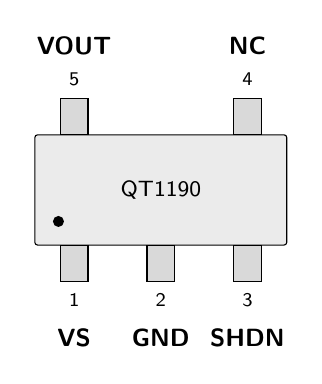
\begin{tikzpicture}[font=\small, pin/.style={fill=black!15, draw, minimum width=0.35cm, minimum height=0.45cm}]
  % package body (SOT-23-5, top view)
  \draw[fill=black!8, rounded corners=1pt] (0,0) rectangle (3.2,1.4);
  \fill (0.3,0.3) circle (0.07);             % pin 1 marker
  \node[font=\footnotesize] at (1.6,0.7) {QT1190};
  % bottom row: pins 1,2,3
  \foreach \x/\n in {0.5/1, 1.6/2, 2.7/3} {
    \node[pin, anchor=north] at (\x,0) {};
    \node[font=\scriptsize, anchor=north] at (\x,-0.5) {\n};
  }
  % top row: pins 5,4
  \foreach \x/\n in {0.5/5, 2.7/4} {
    \node[pin, anchor=south] at (\x,1.4) {};
    \node[font=\scriptsize, anchor=south] at (\x,1.9) {\n};
  }
  % names
  \node[anchor=north, font=\small\bfseries] at (0.5,-0.95) {VS};
  \node[anchor=north, font=\small\bfseries] at (1.6,-0.95) {GND};
  \node[anchor=north, font=\small\bfseries] at (2.7,-0.95) {SHDN};
  \node[anchor=south, font=\small\bfseries] at (0.5,2.3) {VOUT};
  \node[anchor=south, font=\small\bfseries] at (2.7,2.3) {NC};
\end{tikzpicture}
\captionof{figure}{Pin configuration, SOT-23-5 (top view)}
\end{minipage}\hfill
\begin{minipage}[c]{0.56\linewidth}
\small
\begin{tabularx}{\linewidth}{@{}c l X@{}}
  \toprule
  \textbf{Pin} & \textbf{Name} & \textbf{Description} \\
  \midrule
  1 & VS & Supply voltage input, \qty{2.7}{V} to \qty{5.5}{V}; bypass with \qty{100}{nF} \\
  2 & GND & Ground \\
  3 & SHDN & Shutdown input, active low; connect to VS for normal operation \\
  4 & NC & No connection; leave open or connect to GND \\
  5 & VOUT & Analog output, \qty{10}{mV/\celsius} \\
  \bottomrule
\end{tabularx}
\end{minipage}

% ---- Absolute maximum ratings ------------------------------------------------------------
\dsection{Absolute maximum ratings}
Stresses at or above those listed under absolute maximum ratings may cause permanent damage to the device.
These are stress ratings only; functional operation of the device at these or any other conditions above those
indicated in the operational section of this specification is not implied.

\begin{center}
\captionof{table}{Absolute maximum ratings}
\begin{tabular}{@{}l l r@{}}
  \toprule
  \textbf{Parameter} & \textbf{Symbol} & \textbf{Rating} \\
  \midrule
  Supply voltage (VS to GND) & $V_\mathrm{S}$ & \qty{-0.3}{V} to \qty{+6.0}{V} \\
  Shutdown pin voltage & $V_\mathrm{SHDN}$ & \qty{-0.3}{V} to $V_\mathrm{S}$ + \qty{0.3}{V} \\
  Output voltage & $V_\mathrm{OUT}$ & \qty{-0.3}{V} to $V_\mathrm{S}$ + \qty{0.3}{V} \\
  Output current & $I_\mathrm{OUT}$ & \qty{\pm 10}{mA} \\
  Storage temperature range & $T_\mathrm{STG}$ & \qty{-65}{\celsius} to \qty{+150}{\celsius} \\
  Junction temperature & $T_\mathrm{J,max}$ & \qty{150}{\celsius} \\
  Thermal resistance, junction to ambient & $\theta_\mathrm{JA}$ & \qty{190}{\celsius/W} \\
  Lead temperature, soldering (\qty{10}{s}) & & \qty{260}{\celsius} \\
  ESD, human body model & & \qty{2000}{V} \\
  \bottomrule
\end{tabular}
\end{center}

% ---- Electrical characteristics ---------------------------------------------------------------
\Needspace{26\baselineskip}
\dsection{Electrical characteristics}
$V_\mathrm{S}$ = \qty{3.3}{V}, $T_\mathrm{A}$ = \qty{25}{\celsius}, unless otherwise noted. Minimum and maximum
limits are guaranteed by production test; typical values are for information only.

\begin{center}
\small
\captionof{table}{Electrical characteristics}
\begin{tabularx}{\linewidth}{@{}>{\raggedright\arraybackslash}X l c c c c@{}}
  \toprule
  \textbf{Parameter} & \textbf{Test conditions} & \textbf{Min} & \textbf{Typ} & \textbf{Max} & \textbf{Unit} \\
  \midrule
  \multicolumn{6}{@{}l}{\textit{Accuracy}} \\
  Temperature error & $T_\mathrm{A}$ = \qty{25}{\celsius}, grade A & & $\pm$0.5 & $\pm$2.0 & \si{\celsius} \\
  Temperature error & $T_\mathrm{A}$ = \qty{25}{\celsius}, grade B & & $\pm$0.3 & $\pm$1.0 & \si{\celsius} \\
  Temperature error & \qty{-40}{\celsius} to \qty{+125}{\celsius} & & $\pm$1.5 & $\pm$3.0 & \si{\celsius} \\
  Scale factor & \qty{-40}{\celsius} to \qty{+125}{\celsius} & 9.9 & 10.0 & 10.1 & \si{mV/\celsius} \\
  Output voltage at \qty{0}{\celsius} & & 495 & 500 & 505 & \si{mV} \\
  Nonlinearity & \qty{-40}{\celsius} to \qty{+125}{\celsius} & & $\pm$0.2 & & \si{\celsius} \\
  \addlinespace
  \multicolumn{6}{@{}l}{\textit{Output}} \\
  Output impedance & $I_\mathrm{OUT}$ = \qty{0}{mA} to \qty{1}{mA} & & 20 & 35 & \si{\ohm} \\
  Load regulation & $I_\mathrm{OUT}$ = \qty{0}{mA} to \qty{1}{mA} & & 0.1 & 0.4 & \si{\celsius/mA} \\
  Thermal response time & 63\,\% step, still air & & 35 & & \si{s} \\
  \addlinespace
  \multicolumn{6}{@{}l}{\textit{Power supply}} \\
  Supply voltage range & $V_\mathrm{S}$ & 2.7 & & 5.5 & \si{V} \\
  Quiescent current & SHDN = $V_\mathrm{S}$ & & 12 & 20 & \si{\micro A} \\
  Quiescent current & SHDN = $V_\mathrm{S}$, $T_\mathrm{A}$ = \qty{125}{\celsius} & & 17 & 28 & \si{\micro A} \\
  Shutdown current & SHDN = GND & & 0.1 & 1 & \si{\micro A} \\
  Turn-on time & to 1\,\% of final value & & 1.5 & 3 & \si{ms} \\
  \bottomrule
\end{tabularx}
\end{center}

% ---- Typical performance characteristics -----------------------------------------------------
\dsection{Typical performance characteristics}
\begin{center}
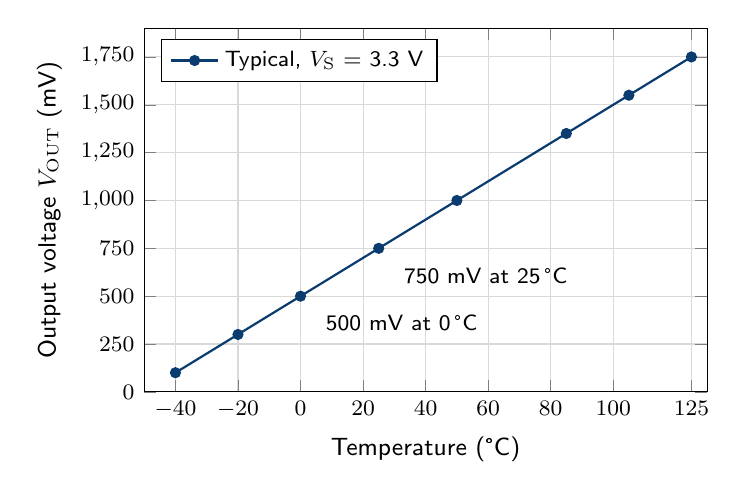
\begin{tikzpicture}
\begin{axis}[
    width=0.72\linewidth, height=6.2cm,
    xlabel={Temperature (\textdegree C)}, ylabel={Output voltage $V_\mathrm{OUT}$ (mV)},
    xmin=-50, xmax=130, ymin=0, ymax=1900,
    xtick={-40,-20,0,20,40,60,80,100,125}, ytick={0,250,500,750,1000,1250,1500,1750},
    grid=both, grid style={black!15}, tick label style={font=\footnotesize}, label style={font=\small},
    legend pos=north west, legend style={font=\footnotesize}]
  \addplot[thick, qblue, mark=*, mark size=1.6pt] coordinates
    {(-40,100) (-20,300) (0,500) (25,750) (50,1000) (85,1350) (105,1550) (125,1750)};
  \addlegendentry{Typical, $V_\mathrm{S}$ = 3.3 V}
  \node[font=\footnotesize, anchor=north west] at (axis cs:30,700) {750 mV at 25\,\textdegree C};
  \node[font=\footnotesize, anchor=north west] at (axis cs:5,450) {500 mV at 0\,\textdegree C};
\end{axis}
\end{tikzpicture}
\captionof{figure}{Output voltage versus temperature}
\end{center}

% ---- Application circuit ------------------------------------------------------------------
\Needspace{16\baselineskip}
\dsection{Applications information}
The QT1190 can be connected directly to the input of a successive-approximation ADC. Place a \qty{100}{nF}
ceramic capacitor close to the supply pin. An RC filter ($R_\mathrm{F}$ and $C_\mathrm{F}$) on the output keeps
the sampling kick-back of the ADC from disturbing the sensor and reduces noise. Keep the SHDN pin at the
supply voltage when the sensor is in use. To measure a temperature, subtract \qty{500}{mV} from the
output voltage and divide by \qty{10}{mV/\celsius}.

\begin{center}
\begin{circuitikz}[scale=0.95, transform shape, american]
  % supply and bypass capacitor
  \draw (0,2.7) node[left]{$V_\mathrm{S}$ = \qty{3.3}{V}} to[short, o-] (2,2.7) to[short, *-] (3.5,2.7);
  \draw (2,2.7) to[C, l_=$C_1$ \qty{100}{nF}] (2,0.4) node[ground]{};
  % sensor
  \draw[fill=black!8] (3.5,1) rectangle (6.5,3);
  \node at (5.0,2.55) {QT1190};
  \node[font=\scriptsize, anchor=west] at (3.55,2.7) {VS};
  \node[font=\scriptsize, anchor=west] at (3.55,2.0) {SHDN};
  \node[font=\scriptsize, anchor=south] at (5.0,1.05) {GND};
  \node[font=\scriptsize, anchor=east] at (6.45,2.0) {VOUT};
  % SHDN tied to VS
  \draw (3.5,2.0) -- (2.8,2.0) to[short, *-] (2.8,2.7);
  % ground
  \draw (5.0,1) -- (5.0,0.4) node[ground]{};
  % output filter and ADC
  \draw (6.5,2.0) to[R, l=$R_\mathrm{F}$ \qty{1}{k\ohm}] (8.5,2.0) to[short, *-o] (10.2,2.0)
        node[right, align=left]{to ADC\\input};
  \draw (8.5,2.0) to[C, l_=$C_\mathrm{F}$ \qty{1}{nF}] (8.5,0.4) node[ground]{};
\end{circuitikz}
\captionof{figure}{Typical application circuit with ADC input filter}
\end{center}

% ---- Ordering information ---------------------------------------------------------------------
\Needspace{12\baselineskip}
\dsection{Ordering information}
\begin{center}
\small
\begin{tabularx}{\linewidth}{@{}l c c c X@{}}
  \toprule
  \textbf{Model} & \textbf{Accuracy at \qty{25}{\celsius}} & \textbf{Package} & \textbf{Marking} & \textbf{Packing} \\
  \midrule
  QT1190AKS-R7 & \qty{\pm 2.0}{\celsius} max & SOT-23-5 & T9A & 7-inch reel, 3000 pieces \\
  QT1190AKS-RL & \qty{\pm 2.0}{\celsius} max & SOT-23-5 & T9A & 13-inch reel, 10000 pieces \\
  QT1190BKS-R7 & \qty{\pm 1.0}{\celsius} max & SOT-23-5 & T9B & 7-inch reel, 3000 pieces \\
  EVAL-QT1190 & & & & Evaluation board with USB interface \\
  \bottomrule
\end{tabularx}
\end{center}
All models are specified for operation from \qty{-40}{\celsius} to \qty{+125}{\celsius} and are
RoHS-compliant. Contact your local Quantro sales office for samples.

\end{document}
